 
\section{Praktika enkonduko}
\subsection{Uzantkontoj}
%%%>>>>>>>>>>>>>>>>>>>>>>>>>>>>>>>>>>>>>>>>>>>>>>>>>>>>>>>>>>>>>>>>>>>>>>>>>>>>>>>>>>>>>>>>>>>>>>
  \begin{frame}
    \frametitle{Ensalutu en trellon}

	Uzu sian propran konton aŭ uzu unu de la subaj:

%	\begin{tabular}{ | c | c | }
%	\hline                       
%		anaso_trejnanto gmail.com & 2anasoj \\
%		alaudo_trejnanto gmail.com & 2alaudoj \\
%		najtingalo_trejnanto gmail.com & 2najgingaloj \\
%		kolombo_trejnanto gmail.com & 2kolomboj\\
%	\hline  
%	\end{tabular}

\end{frame}
%%%<<<<<<<<<<<<<<<<<<<<<<<<<<<<<<<<<<<<<<<<<<<<<<<<<<<<<<<<<<<<<<<<<<<<<<<<<<<<<<<<<<<<<<<<<<<<<<

%%%>>>>>>>>>>>>>>>>>>>>>>>>>>>>>>>>>>>>>>>>>>>>>>>>>>>>>>>>>>>>>>>>>>>>>>>>>>>>>>>>>>>>>>>>>>>>>>
  \begin{frame}
    \frametitle{Fulmklavoj}
    	\begin{columns}
    \column{0.6\textwidth}
	
	Estas malmultaj, sed ege utilaj.
    
	\begin{itemize}
		\item Per klavo ? vi povas rigardi fulmklavaron.
		\item Tre indas tion fari ofte kaj lerni paŝo post paŝo.
	\end{itemize}
    
    	
	\column{0.4\textwidth}
    
    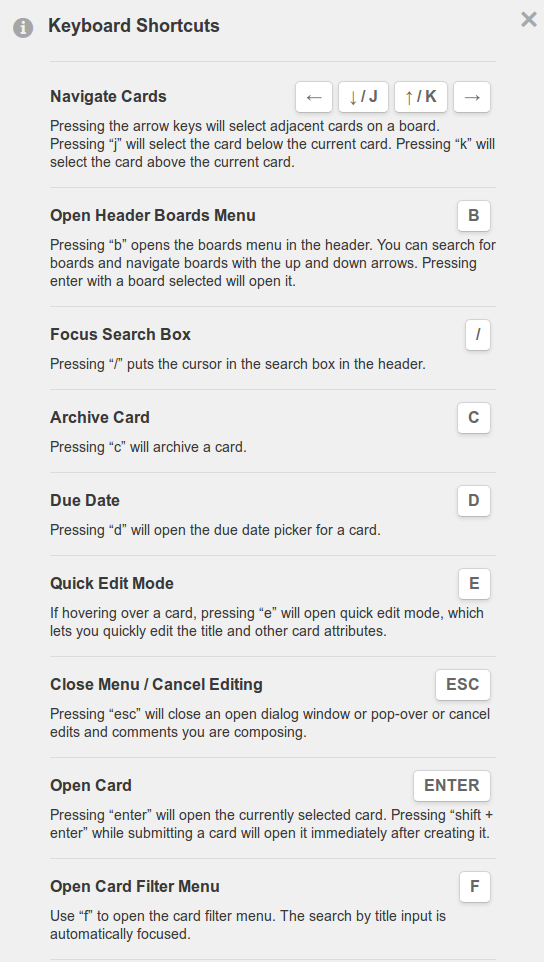
\includegraphics[scale=0.2]{ekranoj/fulmklavaro}
	
	\end{columns}
	
	
  \end{frame}
%%%<<<<<<<<<<<<<<<<<<<<<<<<<<<<<<<<<<<<<<<<<<<<<<<<<<<<<<<<<<<<<<<<<<<<<<<<<<<<<<<<<<<<<<<<<<<<<<




%%%>>>>>>>>>>>>>>>>>>>>>>>>>>>>>>>>>>>>>>>>>>>>>>>>>>>>>>>>>>>>>>>>>>>>>>>>>>>>>>>>>>>>>>>>>>>>>>
  \begin{frame}
    \frametitle{Limdatoj}

    \begin{columns}
    \column{0.6\textwidth}
    
    Tre utilas. Oni ankaŭ ricevas sciigon unu tago antaŭ ĝi.
    
    	
	\column{0.4\textwidth}
    
    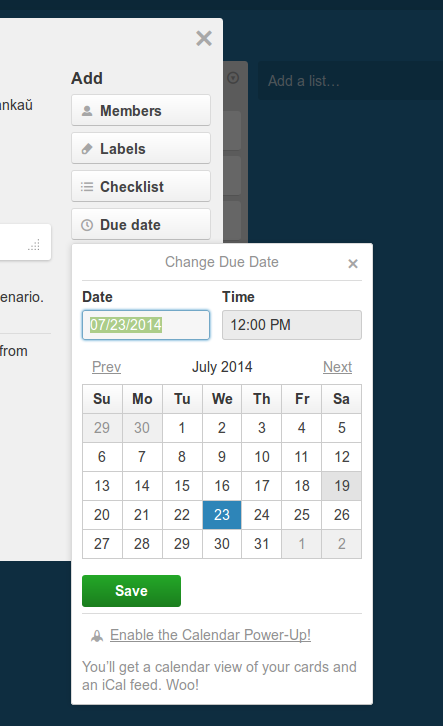
\includegraphics[scale=0.2]{ekranoj/limdato}
	
	\end{columns}
	
	
	
  \end{frame}
%%%<<<<<<<<<<<<<<<<<<<<<<<<<<<<<<<<<<<<<<<<<<<<<<<<<<<<<<<<<<<<<<<<<<<<<<<<<<<<<<<<<<<<<<<<<<<<<<



%%%>>>>>>>>>>>>>>>>>>>>>>>>>>>>>>>>>>>>>>>>>>>>>>>>>>>>>>>>>>>>>>>>>>>>>>>>>>>>>>>>>>>>>>>>>>>>>>
  \begin{frame}
    \frametitle{Nomo de kartoj}
		
	Trello havas tre potencan serĉilon. La nomo estu ŝerĉebla post du jaroj.
	
	Ezkemple, anstataŭ "Paperaĵoj" uzu "Pruviloj de la vojaĝo al Italio".
  \end{frame}
%%%<<<<<<<<<<<<<<<<<<<<<<<<<<<<<<<<<<<<<<<<<<<<<<<<<<<<<<<<<<<<<<<<<<<<<<<<<<<<<<<<<<<<<<<<<<<<<<



%%%>>>>>>>>>>>>>>>>>>>>>>>>>>>>>>>>>>>>>>>>>>>>>>>>>>>>>>>>>>>>>>>>>>>>>>>>>>>>>>>>>>>>>>>>>>>>>>
  \begin{frame}
    \frametitle{Markolistoj}
		
		\begin{center}
		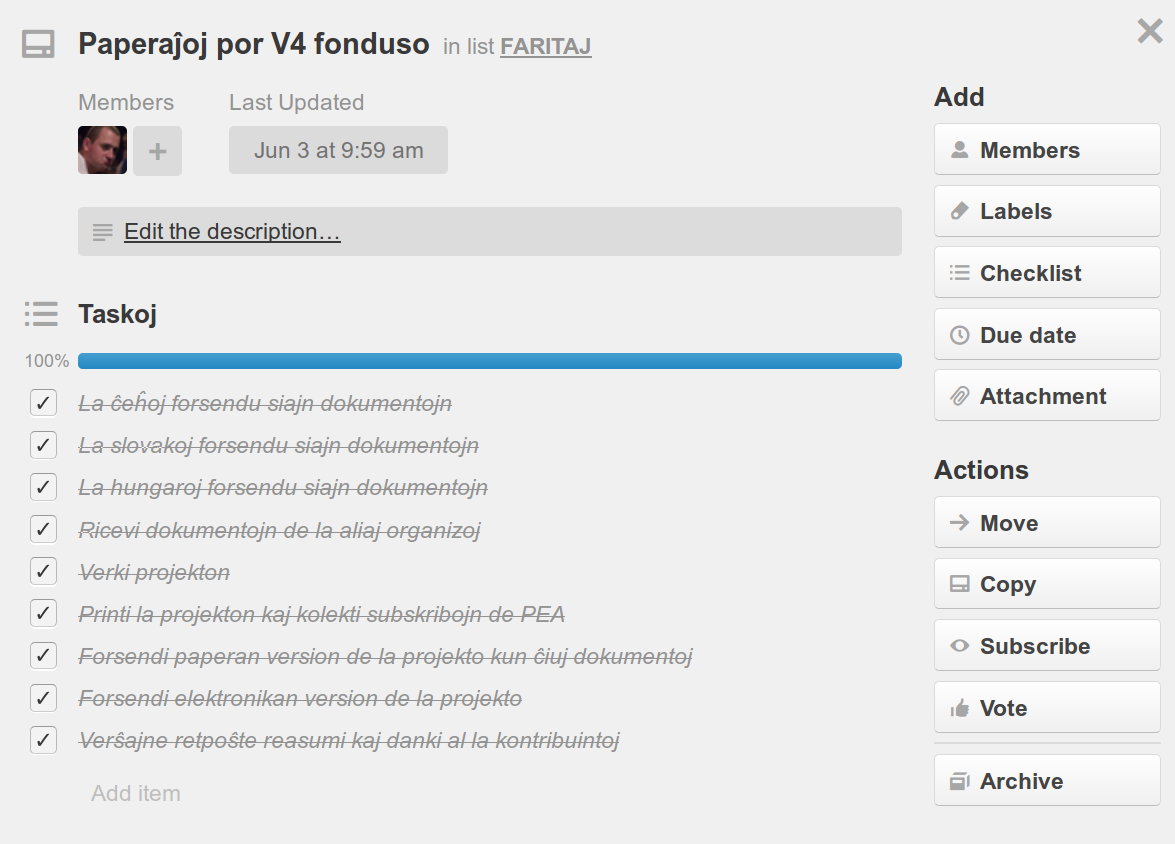
\includegraphics[scale=0.222]{ekranoj/markolistoj}
		\end{center}
	
  \end{frame}
%%%<<<<<<<<<<<<<<<<<<<<<<<<<<<<<<<<<<<<<<<<<<<<<<<<<<<<<<<<<<<<<<<<<<<<<<<<<<<<<<<<<<<<<<<<<<<<<<



%%%>>>>>>>>>>>>>>>>>>>>>>>>>>>>>>>>>>>>>>>>>>>>>>>>>>>>>>>>>>>>>>>>>>>>>>>>>>>>>>>>>>>>>>>>>>>>>>
  \begin{frame}
    \frametitle{Markolistoj + Mencioj}
    
	\begin{center}
    	Atentu: \alert{tio ne produktas sciigojn!}
	\end{center}
		
	\begin{center}
		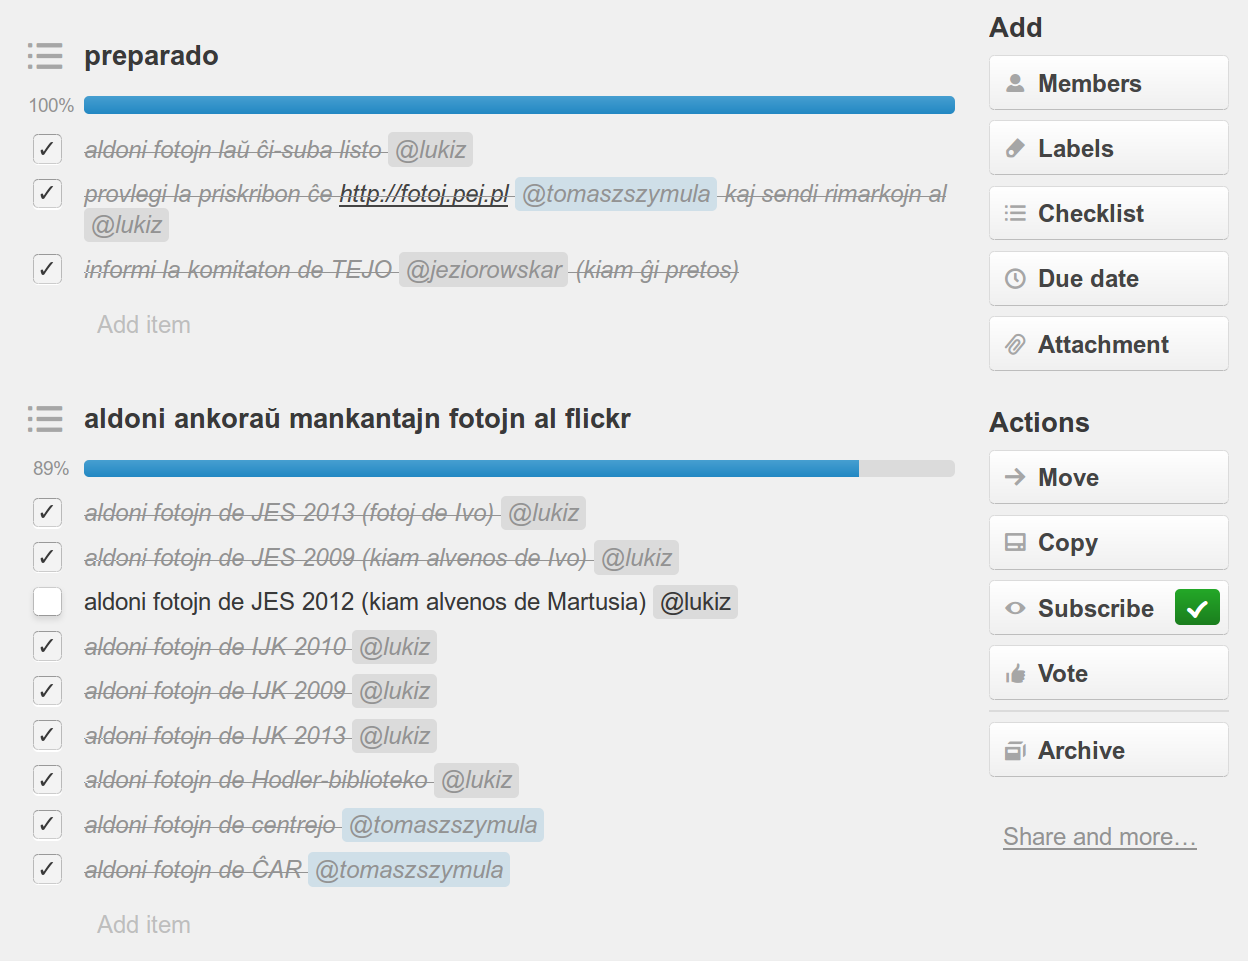
\includegraphics[scale=0.175]{ekranoj/markolistoj-kun-mencioj}
	\end{center}
	
  \end{frame}
%%%<<<<<<<<<<<<<<<<<<<<<<<<<<<<<<<<<<<<<<<<<<<<<<<<<<<<<<<<<<<<<<<<<<<<<<<<<<<<<<<<<<<<<<<<<<<<<<


\subsection{Para klakado}
%%%>>>>>>>>>>>>>>>>>>>>>>>>>>>>>>>>>>>>>>>>>>>>>>>>>>>>>>>>>>>>>>>>>>>>>>>>>>>>>>>>>>>>>>>>>>>>>>
  \begin{frame}
    \frametitle{Pariĝu!}
    Decidu kiu unue estos gufujdijhoranto, kiu gufujkliento.
    
    Ambaŭ personoj havu iun ajn aliron al Trello: telefono, tableto aŭ komputilo. Prefere samtempe, se mankos iloj ni atendos ghis chiuj paroj finos.
    
    Flanka peto: ne malpurigu la komputilojn! :-)
    
  \end{frame}
%%%<<<<<<<<<<<<<<<<<<<<<<<<<<<<<<<<<<<<<<<<<<<<<<<<<<<<<<<<<<<<<<<<<<<<<<<<<<<<<<<<<<<<<<<<<<<<<<

%%%>>>>>>>>>>>>>>>>>>>>>>>>>>>>>>>>>>>>>>>>>>>>>>>>>>>>>>>>>>>>>>>>>>>>>>>>>>>>>>>>>>>>>>>>>>>>>>
  \begin{frame}
    \frametitle{Ekzerco}

	\begin{itemize}
		\item Diĵoranto:
		\begin{enumerate}
			\item Kreu tabulon "Posttagmeza menuo".
			\item Agordu tiel, ke nuraj listoj estu: MENDOJ, SERVITAJ, MENUO.
			\item Aldonu du kartojn: "Obleo kun dolĉa ŝmiraĵo", "Teo".
			\item Aldonu la klienton al la tabulo.
		\end{enumerate}
			
		\item Kliento:
		\begin{enumerate}
			\item Mendu dolĉaĵon (kreu taŭgan karton en la taŭga listo).
			\item Aldonu la diĵoranton al la karto.
		\end{enumerate}    
	\end{itemize}
	    
  \end{frame}
%%%<<<<<<<<<<<<<<<<<<<<<<<<<<<<<<<<<<<<<<<<<<<<<<<<<<<<<<<<<<<<<<<<<<<<<<<<<<<<<<<<<<<<<<<<<<<<<<

%%%>>>>>>>>>>>>>>>>>>>>>>>>>>>>>>>>>>>>>>>>>>>>>>>>>>>>>>>>>>>>>>>>>>>>>>>>>>>>>>>>>>>>>>>>>>>>>>
  \begin{frame}
    \frametitle{Ekzerco2}

	\begin{itemize}
			
		\item Diĵoranto:
		\begin{enumerate}
			\item Kreu markoliston kun jenaj paŝoj:
				\begin{enumerate}
					\item Difini kia ŝmiraĵo
					\item Servado
					\item Pagado
				\end{enumerate}
				
			\item Demandu kia ŝmiraĵo kaj metu klienton sur la karto.
		\end{enumerate}
				
    
		\item Kliento:
		\begin{enumerate}
			\item Respondu pri ŝmiraĵo, marku ĝustan paŝon sur la markolisto.
			\item Remetu diĵoranton al la karto.
		\end{enumerate}    
		
		\item Diĵoranto:
		\begin{enumerate}
			\item Servu, marku markoliston.
			\item Metu la karton en "SERVITAJ" listo.
		\end{enumerate}    
			
	\end{itemize}		
	
    
  \end{frame}
%%%<<<<<<<<<<<<<<<<<<<<<<<<<<<<<<<<<<<<<<<<<<<<<<<<<<<<<<<<<<<<<<<<<<<<<<<<<<<<<<<<<<<<<<<<<<<<<<


%%%>>>>>>>>>>>>>>>>>>>>>>>>>>>>>>>>>>>>>>>>>>>>>>>>>>>>>>>>>>>>>>>>>>>>>>>>>>>>>>>>>>>>>>>>>>>>>>
  \begin{frame}
    \frametitle{Esenco}
    
	Vi ĉiam strebu \alert{forigi sian vizaĝon de la karto} per:
    
    \begin{itemize}
    	\item plenumo de la peto/tasko,
    	\item klarigo kial ne vi taŭgas (ĉiam trovu anstataŭanton),
    	\item aliaj laŭ via kreemeco, kondiĉe ke kun \alert{fortaj argumentoj} por tio.
    \end{itemize}
    
  \end{frame}
%%%<<<<<<<<<<<<<<<<<<<<<<<<<<<<<<<<<<<<<<<<<<<<<<<<<<<<<<<<<<<<<<<<<<<<<<<<<<<<<<<<<<<<<<<<<<<<<<

